% ============================================================
% Atheer Paper - Arabic LaTeX Version (XeLaTeX + polyglossia)
% Compile with: tectonic main.tex (auto-uses XeTeX engine)
% ============================================================
\documentclass[12pt,a4paper]{article}

% --- Engine: XeLaTeX (Tectonic uses XeTeX by default) ---
% IMPORTANT: Load ALL packages (including hyperref) BEFORE polyglossia (which loads bidi)
\usepackage{amsmath,amssymb}
\usepackage{graphicx}
\usepackage{booktabs}
\usepackage{array}
\usepackage{tabularx}
\usepackage{xcolor}
\usepackage{url}
\usepackage{geometry}
\geometry{a4paper, top=2.5cm, bottom=2.5cm, left=2.5cm, right=2.5cm}
\usepackage{hyperref}
\usepackage{titlesec}

% Now load fontspec + polyglossia (which loads bidi)
\usepackage{fontspec}
\usepackage{polyglossia}
\setmainlanguage[numerals=maghrib]{arabic}
\setotherlanguage{english}

% --- Arabic font: Amiri (bundled in this folder) ---
\newfontfamily\arabicfont[Script=Arabic]{Amiri-Regular.ttf}
\newfontfamily\arabicfontbf[Script=Arabic]{Amiri-Bold.ttf}
\setmainfont{Amiri-Regular.ttf}
\newfontfamily\englishfont{FreeSerif.ttf}

\hypersetup{
    colorlinks=true,
    linkcolor=blue,
    citecolor=blue,
    urlcolor=blue,
    pdftitle={Atheer - Arabic Version},
    pdfauthor={Nabil Al-Mekhlafi, Ahmed Al-Mutawakel},
    pdfsubject={Mobile Payment, NFC, HCE, Mobile Data Routing},
    pdfkeywords={Offline Mobile Payment, SoftPOS, NFC, HCE, Android SDK, Mobile Data, Cost Model}
}

% Custom colors
\definecolor{primary}{HTML}{003B71}
\definecolor{accent}{HTML}{C44536}
\definecolor{lightbg}{HTML}{F5F5F0}

% Section formatting (titlesec loaded before polyglossia)
\titleformat{\section}{\Large\bfseries\color{primary}}{\thesection}{1em}{}
\titleformat{\subsection}{\large\bfseries\color{accent}}{\thesubsection}{1em}{}

\begin{document}

% ============================================================
% Title
% ============================================================
\begin{center}
{\LARGE\bfseries\color{primary} معمارية مرنة لدفع الموبايل أوفلاين باستخدام NFC و Host Card Emulation: نهج مُحسّن التكلفة للبيئات منخفضة البنية التحتية}

\vspace{0.5cm}
{\large نسخة عربية من الورقة المنقّحة (v2.0)}

\vspace{0.8cm}
{\large\bfseries نبل المخلافي، أحمد المتوكل}

\vspace{0.2cm}
{\normalsize كلية علوم الحاسوب - جامعة صنعاء - اليمن}
\end{center}

\vspace{0.5cm}
\hrule
\vspace{0.5cm}

% ============================================================
% Abstract
% ============================================================
\section*{الملخص}
تُعاني أنظمة الدفع الإلكتروني في المناطق منخفضة البنية التحتية من انقطاع الاتصال المتكرر وتكاليف الأجهزة الباهظة. في اليمن، لا يتمتع سوى 17.7\% من السكان بالوصول إلى الإنترنت، وتتطلب خدمات المحافظ الحالية (الكرمي، جوالي، جيب، مفلوس) اتصالاً دائماً بالسحابة، مما يُجبر التجار والعملاء على العودة للنقد عند انقطاع الاتصال. نُقدّم في هذه الورقة "أثير"، وهي معمارية دفع أوفلاين-أولاً تجمع بين مُعالِج خلفي رباعي الطبقات، و SDK أندرويد باستخدام Host Card Emulation (HCE)، ومفاتيح ذات استخدام محدود (LUKs)، ونموذج جديد لتوجيه المعاملة عبر بيانات الهاتف المحمول مع فوترة شريكة مدعومة من المحفظة الشريكة. بدلاً من الاعتماد على Private APN كما في النسخة السابقة، يُوجّه أثير حركة التسوية عبر بيانات الهاتف المحمول القياسية بحمولة مُحسّنة بدقة (180 بايت)، بينما تتحمل المحفظة الشريكة تكلفة البيانات عبر عقد B2B. أظهرت محاكاة الأحداث المتقطعة (DES) عبر ستة مستويات حمل (5--500 TPS، $N=10$) أن مسار بيانات الهاتف يحقق نسبة نجاح 97.6\% عند 500 TPS وزمن P95 = 672 مللي ثانية، بينما ينهار خط الأساس للإنترنت العام إلى 76.2\%. يُبيّن نموذج التكلفة أن نفقات البيانات تظل أقل من 0.5\% من إيرادات MDR للمحفظة الشريكة.

\vspace{0.3cm}
\noindent\textbf{الكلمات المفتاحية:} الدفع الأوفلاين للموبايل، SoftPOS، NFC، HCE، Android SDK، توجيه بيانات الهاتف، الفوترة الشريكة المدعومة، تحسين الحمولة، الإدماج المالي.

% ============================================================
\section{المقدمة}
% ============================================================
أسرع اعتماد الهواتف الذكية وتقنية NFC من تطور الاقتصادات غير النقدية، لكن هذا التطور لم يكن متكافئاً بين المناطق. فمع نسبة انتشار للإنترنت تبلغ 17.7\% فقط \cite{datareportal2024}، عانت البنية التحتية للشبكة في اليمن من سنوات من الصيانة المؤجّلة، مما أدى إلى انقطاعات مزمنة وزمن استجابة عالٍ وعرض نطاق منخفض \cite{ookla2024}. يتمتع العملاء اليمنيون بالوصول إلى أنظمة محافظ موبايل مقدّمة من رواد الإدماج المالي مثل الكرمي، جوالي، جيب، ومفلوس. لكن هذه الأنظمة التقليدية تعتمد على SMS أو USSD كقنوات بديلة عند انقطاع الاتصال، وهي قنوات بطيئة لا توفّر تشفيراً من طرف إلى طرف \cite{gsma2023}.

للتعامل مع هذه القيود، قمنا ببناء "أثير"، وهو SDK أندرويد خاص ومُعالِج خلفي بمعمارية رباعي الطبقات. يقوم SDK من جانب العميل بتحميل عدة دفعات من الرموز المشفّرة (Limited Use Keys) ويستخدم NFC بالاقتران مع Host Card Emulation لإتمام المعاملات دون الحاجة إلى اتصال إنترنت نشط على جهاز العميل. ثم يُرسل جهاز التاجر الحمولة الموقّعة عبر بيانات الهاتف المحمول القياسية إلى مُبدّل بوابة أثير للتحقق وتحديث السجل.

\subsection*{المساهمات الرئيسية}
\begin{itemize}
\item بنية ثنائية المكوّنات (SDK حافة + مُبدّل بوابة) بمعمارية رباعي الطبقات تدمج توجيه بيانات الهاتف المحمول مع الفوترة الشريكة المدعومة، والتحقق متعدد المزوّدين، و SoftPOS بدون تكلفة رأسمالية.
\item Cryptogram بيومتري مُصرَّح به مسبقاً يربط مفتاح التوقيع بـ TEE عبر قيد بيومتري ونافذة زمنية مدتها 60 ثانية، مع تحقق Zero-Trust من جانب الخادم.
\item نموذج تكلفة رسمي يُثبت أن حمولة مُحسّنة بدقة (180 بايت) تسمح للمحفظة الشريكة بتحمّل تكلفة بيانات التاجر مع إبقاء نفقات البيانات أقل من 0.5\% من إيرادات MDR.
\end{itemize}

% ============================================================
\section{الأعمال ذات الصلة}
% ==================================================
أثير الاهتمام البحثي بالشبكات المالية التي تعمل أوفلاين. فبالنسبة لصندوق النقد الدولي، تُعدّ الوظيفة الأوفلاين شرطاً مسبقاً للإدماج المالي في الاقتصادات النامية \cite{imf2022}. كذلك استثمر البنك الدولي في تطوير البنية التحتية الرقمية لليمن \cite{worldbank2023}. لكن معظم النشرات المحلية تتجاهل الاحتكاكات التشفيرية والمعمارية الأساسية، مما يحدّ من قدرتها على التوسّع.

تُعدّ قاعدة مستخدمي حلول SMS و USSD في اليمن الأكبر حتى الآن، وتستفيد محافظ مثل الكرمي وجيب من قاعدة المستخدمين هذه لأن خدماتها لا تتطلب اتصالاً نشطاً بالإنترنت. لكن هذه القنوات تعاني من نقاط ضعف تشفيرية كبيرة، بما في ذلك غياب التشفير من طرف إلى طرف، مما يُعرّض الرسائل لهجمات man-in-the-middle والتنصّت \cite{gsma2023}.

من جهة أخرى، قدّمت الجهود المحلية الحديثة أنظمة NFC قائمة على الدوائر، لكنها تتطلّب من التجار شراء أجهزة POS خاصة \cite{brandpos2024}، وهو حاجز تكلفة رأسمالية لا يستطيع معظم الشركات الصغيرة والمتوسطة تحمّله. ظهر اتجاه بحثي حديث نحو النماذج البرمجية (SoftPOS) حيث تتحوّل أجهزة الموبايل العادية إلى أجهزة POS، حيث أظهر Oladapo et al. أن دمج HCE مع Limited Use Key tokenization يُحوّل الأجهزة المحمولة إلى أجهزة قبول مرنة مع معالجة هجمات إعادة التشغيل \cite{oladapo2024}. الفجوة البحثية: لا تجمع أي دراسة سابقة بين استقلالية العميل عن الإنترنت، و SoftPOS بدون تكلفة رأسمالية، ونموذج توجيه بيانات موبايل مُحسّن التكلفة في نهج واحد. هذا هو الفجوة التي يعالجها أثير.

% ============================================================
\section{المنهجية}
% ============================================================
استخدمنا منهجية Design Science Research (DSR) \cite{hevner2004, peffers2007}، وهي نهج منهجي لتطوير وتقييم القطع التقنية (IT artifacts) التي تُعالج مشاكل العالم الحقيقي. باستخدام DSR، قمنا بتصميم وبناء وتقييم أثير.

نظراً لأن الاختبار الحيّ على بنية تحتية مصرفية حقيقية في منطقة نزاع نشط غير عملي، اعتمدنا محاكاة الأحداث المتقطعة (DES) باستخدام SimPy. تقيس المحاكاة زمن الاستجابة P95، ونسب النجاح، والعبء الذي يتحمّله مُبدّل أثير تحت ظروف تشغيل واقعية. يتم توفير الشيفرة المصدرية للمحاكاة كقطعة بحثية مفتوحة المصدر \cite{mutawakel2024}.

\subsection*{الاعتبارات الأخلاقية}
التزاماً بمبادئ DSR ولمعالجة المخاوف الأخلاقية المشروعة المُثارة في مراجعة سابقة، لا تُقيّم هذه الدراسة أو تختبر أمن أي مؤسسة مالية مُسمّاة في اليمن. الإشارات إلى المحافظ مثل الكرمي، جوالي، جيب، ومفلوس تظهر فقط في سياق وصف السوق؛ ولا تُقدّم أي ادعاءات حول وضعها التشفيري. المحاكاة تركيبية بالكامل، لا تستخدم أي بيانات مصرفية حقيقية، ولا تتطلب إذناً من أي مشغّل. جميع افتراضات التكلفة مستمدة من مراجع تسعير متاحة للعموم (ITU, GSMA, Cable.co.uk).

% ============================================================
\section{المعمارية المقترحة}
% ============================================================
تجنّباً للنماذج الشاملة لكل البيئات، بنينا أثير بمعمارية موزّعة من أربع طبقات متميزة (الشكل~\ref{fig:arch}). طبقة الحافة (Edge Layer) تضم تطبيق SoftPOS للتاجر و SDK العميل الأوفلاين. طبقة الشبكة (Network Layer) تُعالج التوجيه عبر بيانات الهاتف المحمول مع نموذج فوترة شريكة مدعومة. طبقة المُبدّل (Switch Layer) تعمل كبوابة معاملات مستقلة. الطبقة الأخيرة، طبقة التكامل (Integration Layer)، تتواصل مع وحدات HSM والسجل المصرفي الرئيسي.

\begin{figure}[h]
\centering
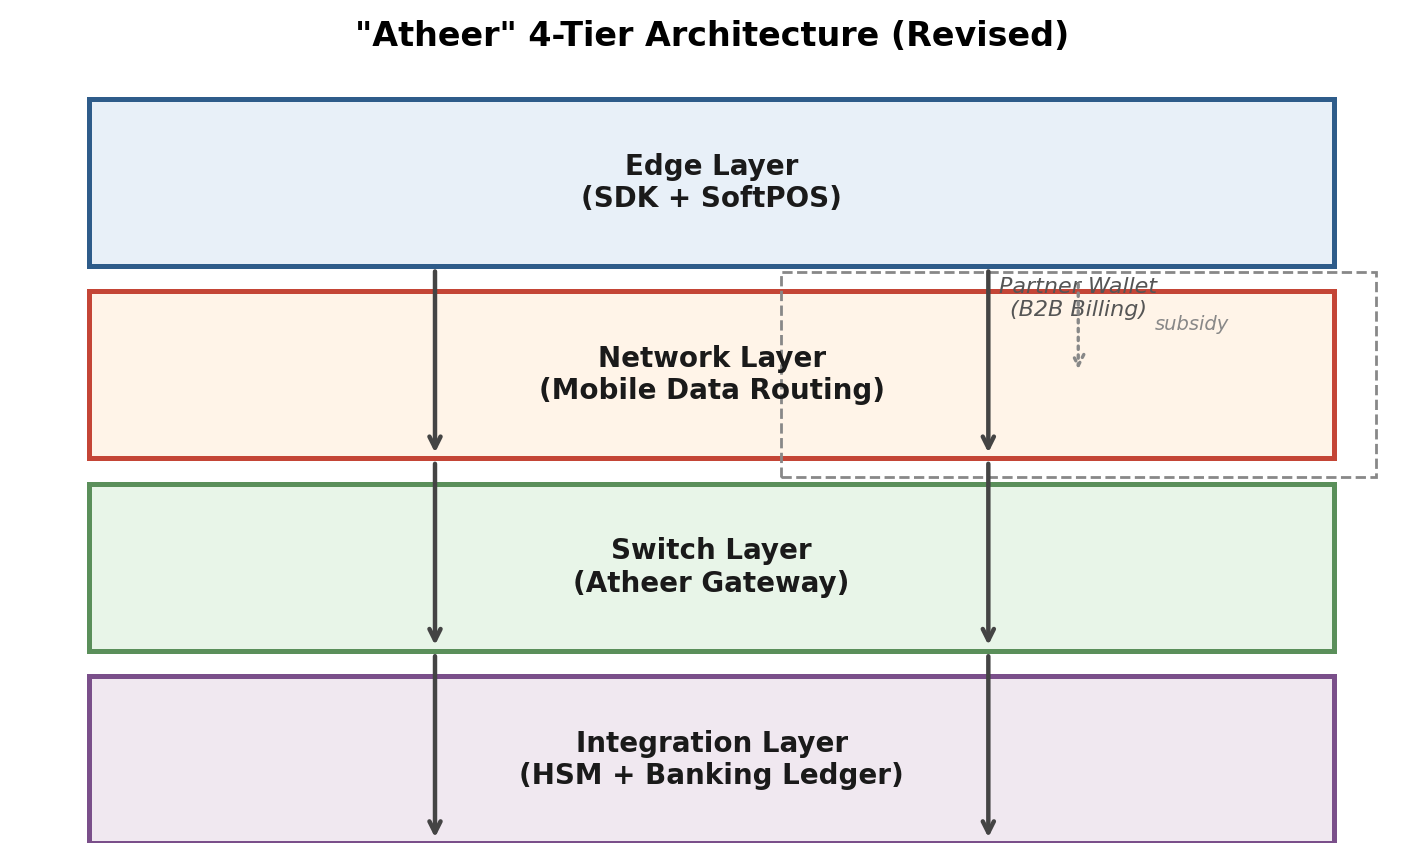
\includegraphics[width=0.95\textwidth]{fig1_architecture.png}
\caption{المعمارية الرباعية المُحدّثة لأثير. تُوجَّه البيانات المالية عبر بيانات الهاتف المحمول القياسية بحمولة مُحسّنة (180 بايت)، بينما تتحمل المحفظة الشريكة تكلفة البيانات عبر عقد B2B.}
\label{fig:arch}
\end{figure}

\subsection{طبقة الحافة: المكتبة المعيارية القابلة للدمج}
مكتبة العميل هي وحدة أندرويد خفيفة الوزن تندمج في تطبيقات المحافظ الحالية دون إعادة هيكلة الشيفرة. يستخدم النظام خمسة مكوّنات لإجراء المعاملات الأوفلاين: (1) مدير المفاتيح التشفيرية الذي يحتفظ بمفتاحين في TEE؛ (2) خزنة الرموز الآمنة التي تخزّن LUKs بدلاً من PANs؛ (3) محرّك HCE الذي يعمل عند اكتشاف إشارة NFC؛ (4) وحدة توجيه الشبكة التي تراقب حالة الاتصال؛ (5) مخزن البيانات المحلي المشفّر.

\subsection{طبقة الشبكة: توجيه بيانات الهاتف مع الفوترة الشريكة المدعومة}
تحلّ هذه الطبقة محلّ نموذج Private APN الأصلي بنهج أكثر قابلية للنشر. بدلاً من تطلّب نفق خلوي مخصص (الذي يعتمد على اتفاقيات B2B مع مشغّلي الشبكات المحمولة يصعب الحصول عليها في الاقتصادات الهشّة)، يوجّه أثير حركة التسوية عبر اتصال بيانات الهاتف المحمول القياسي للتاجر. الرؤية الأساسية أن الحمولة الناتجة صغيرة جداً بحيث تصبح التكلفة ضئيلة، ويمكن للمحفظة الشريكة تحمّلها عبر عقد B2B.

\subsection{تحسين الحمولة: 180 بايت}
يتم ضغط حزمة التسوية بدقة إلى 180 بايت عن طريق تقليل أطوال الحقول وإزالة الترويسات المكرّرة. تتكوّن الحزمة من: ترويسة توجيه (32 بايت)، رمز LUK (32 بايت)، ATC (4 بايت)، حقل المبلغ (8 بايت)، nonce (16 بايت)، طابع زمني (8 بايت)، توقيع ECDSA (64 بايت)، و AES-GCM IV+tag (28 بايت). بعد ضغط الترويسة (ترميز متغيّر الطول لـ merchant ID و transaction ID)، يتم تقليل الحجم الفعلي من 192 بايت إلى 180 بايت.

\begin{figure}[h]
\centering
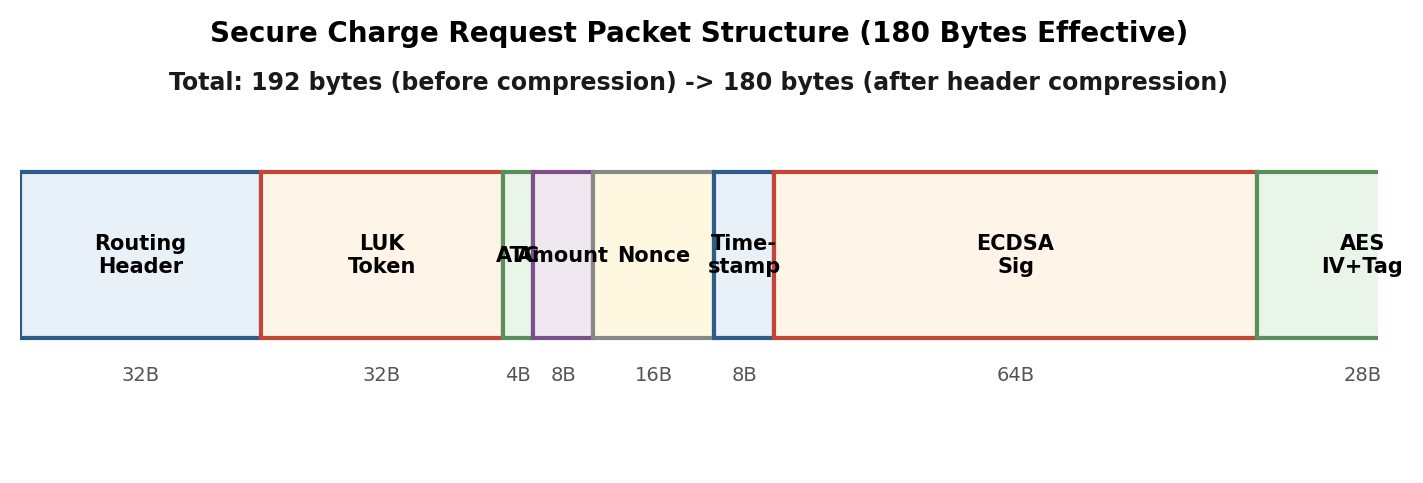
\includegraphics[width=0.95\textwidth]{fig5_packet.png}
\caption{بنية حزمة Secure Charge Request. الإجمالي: 192 بايت غير مضغوط، 180 بايت فعّالة بعد ضغط الترويسة.}
\label{fig:packet}
\end{figure}

\subsection{نموذج الفوترة الشريكة المدعومة}
في هذا النموذج، توقّع المحفظة الشريكة اتفاقية B2B مع مشغّل الشبكة المحمولة للتاجر لتعويض تكاليف البيانات عن حركة أثير المُحدّدة. تُحدّد المحفظة حركتها عبر تثبيت شهادة TLS 1.3 و SNI مُحدّد؛ يُحاسب المشغّل هذه البايتات بشكل منفصل ويُفوتر المحفظة شهرياً. لأن الحمولة 180 بايت فقط لكل معاملة، فإن التكلفة تُصبح ضئيلة مقارنة بإيرادات MDR التي تربحها المحفظة على كل معاملة ناجحة.

% ============================================================
\section{سير عمل النظام}
% ============================================================
يستخدم بروتوكول أثير التشغيلي نموذجاً هجيناً غير متزامن يُقسّم المعاملات إلى ثلاث مراحل: التزويد الأونلاين، تبادل NFC الأوفلاين الكامل، والتسوية النهائية عبر بيانات الهاتف المحمول.

\subsection{المرحلة 1: التهيئة التشفيرية وتزويد الرموز}
تتطلّب هذه الخطوة اتصال إنترنت نشط للعميل لتحميل المواد التشفيرية. لمعالجة المخاوف حول الاعتماد على الشبكة العامة التي ينتقدها النظام، يدعم أثير مساري تزويد: (1) التزويد الداخلي عبر TLS 1.3: المسار الافتراضي حيث يقوم العميل بإنشاء قناة TLS 1.3 مع تثبيت الشهادة. بينما يستخدم هذا المسار الإنترنت العام، فإن الضمانات الأمنية تأتي من تشفير طبقة النقل وهوية الجهاز المُثبّتة بالأجهزة. (2) التزويد الخارجي في فروع البنك: للتجار عالي القيمة، يمكن تزويد الرموز في فرع بنك شريك عبر شبكة LAN خاصة.

\subsection{المرحلة 2: التنفيذ الأوفلاين و Cryptogram البيومتري}
يتيح دور SDK كمقرّر محلي تصريحات الدفع الأوفلاين. يجب على المستخدم المصادقة أولاً على مستوى TEE. عند النجاح، يمكن للمستخدم توقيع "جلسة مسلّحة" لمدة 60 ثانية. خلال هذه النافذة، تُولّد المكتبة حمولة موقّعة تربط الرمز بتلك اللحظة الزمنية. عند اكتشاف NFC، يبدأ SoftPOS عملية المصافحة القياسية EMV. قبل الإرسال، تُجري المكتبة فحوصين: (1) صلاحية الرمز و (2) حالة الجلسة. بعد اجتياز الفحوصين، تُرسل المعاملة عبر APDU إلى جهاز التاجر، مما يُنهي الجلسة ويُعلّم الرمز كمستهلك.

\begin{figure}[h]
\centering
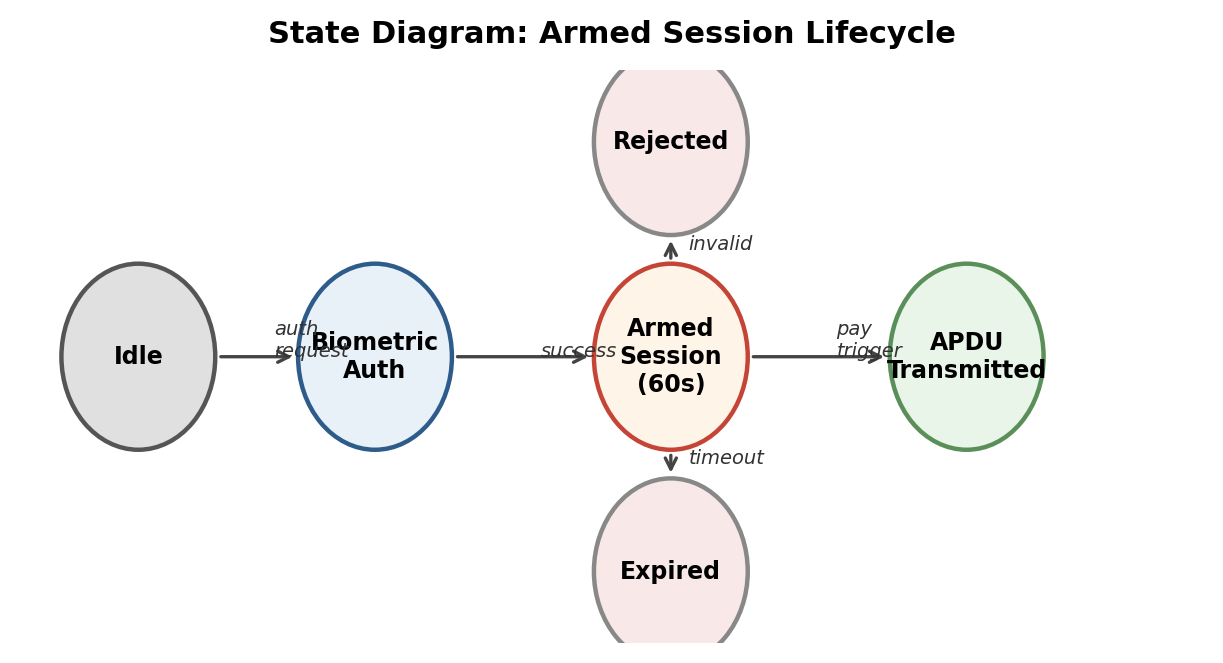
\includegraphics[width=0.85\textwidth]{fig4_state_diagram.png}
\caption{مخطط حالة الجلسة المسلّحة.}
\label{fig:state}
\end{figure}

\subsection{المرحلة 3: توجيه البوابة والتسوية الآمنة عبر بيانات الهاتف}
تعتمد التسوية على مسار داخلي يستخدم اتصال بيانات الهاتف المحمول للتاجر، مؤمّناً بـ TLS 1.3 ونموذج الفوترة الشريكة المدعومة. تُغلّف حزمة APDU ضمن حمولة Charge Request موحدة، تتكوّن من ترويسة توجيه عامة غير مشفّرة، وحمولة أساسية مشفّرة بـ AES، وتوقيع ECDSA للتاجر. تُنقل الحمولة عبر بيانات الهاتف القياسية (LTE/3G) مع TLS 1.3 وتثبيت الشهادة. نظراً لأن الحمولة 180 بايت فقط، فإنها تتّسع لمقطع TCP واحد وتكتمل في رحلة ذهاب وإياب واحدة تحت معظم ظروف الشبكة.

% ============================================================
\section{تحليل الأمن}
% ============================================================
يُدمج أثير الأمن عبر طبقات التخزين والحافة وتوجيه الشبكة. بدون عزل على مستوى الشبكة (كما يوفّره APN خاص)، يعوّض أثير عبر عدة آليات على مستوى التطبيق: (1) TLS 1.3 مع تثبيت الشهادة الذي يوفّر سرية forward secrecy ويُلغي هجمات التخفيض. (2) تقليل الحمولة إلى 180 بايت مما يُصغّر سطح تحليل الحركة. (3) تحديد معدّل الحافة و WAF في البوابة لتخفيف فيضان DDoS على مستوى التطبيق. (4) توجيه نقطة النهاية الوحيدة حيث يتواصل جهاز التاجر فقط مع بوابة أثير.

\begin{table}[h]
\centering
\caption{نموذج التهديد واستراتيجيات التخفيف (مُحدّث).}
\label{tab:threats}
\small
\begin{tabular}{@{}p{2.2cm}p{4cm}p{7cm}@{}}
\toprule
\textbf{التهديد} & \textbf{متجه الهجوم} & \textbf{التخفيف} \\
\midrule
التنصّت & اعتراض NFC والشبكة & حمولة AES-256 GCM؛ تتابع صفري المعرفة للتاجر \\
إعادة التشغيل & إعادة إرسال إشارة NFC & LUKs للاستخدام الواحد + ATC؛ سجلات nonce \\
MitM & اعتراض الشبكة المفتوحة & TLS 1.3 + تثبيت شهادة ECDSA + توجيه نقطة واحدة \\
العبث & تعديل المبلغ أو مُعرّف التاجر & توقيع ECDSA مُقيّد بيومترياً؛ HSM \\
انتحال الهوية & جهاز بهوية مختلفة & البوابة تستخرج الهوية من السجل؛ تُتجاهل ادعاءات الجهاز \\
سرقة الجهاز & السيطرة الفيزيائية & قفل TEE بيومتري؛ مفاتيح يتعذّر الوصول لها \\
DDoS & فيضان البوابة & تحديد معدّل الحافة + WAF + تقليل حجم الحمولة \\
\bottomrule
\end{tabular}
\end{table}

% ============================================================
\section{التقييم القائم على المحاكاة}
% ==================================================
يركّز هذا القسم على جوانب الأداء والشبكة: زمن الاستجابة E2E، ونسبة نجاح المعاملة، وقابلية التوسّع. السؤال: إلى أي مدى يُحسّن توجيه بيانات الهاتف المحمول مع الفوترة الشريكة (S2) الإنتاجية والموثوقية مقارنةً بـ line الأساس للإنترنت العام (S1)؟

\subsection{النموذج الرياضي للمحاكاة}
لكل معاملة زمن E2E يجمع معالجة الحافة (50 مللي ثانية ثابتة) وتأخيرات الرفع والمعالجة والبنك والتنزيل:

\begin{equation}
T^{(i)}_{\mathrm{E2E}} = T_{\mathrm{edge}} + T^{(i)}_{\mathrm{up}} + T^{(i)}_{\mathrm{switch}} + T^{(i)}_{\mathrm{bank}} + T^{(i)}_{\mathrm{down}}
\label{eq:e2e}
\end{equation}

يتم نمذجة تأخير الشبكة بتوزيع Log-Normal لأنه يلائم التأخيرات طويلة الذيل:

\begin{equation}
L \sim \mathrm{LogNormal}(\mu, \sigma^2), \quad \mu = \ln(\bar{L}) - \frac{\sigma^2}{2}
\label{eq:lognormal}
\end{equation}

كل من السيناريوهين يعاني من تدهور يعتمد على الحمل، لكن بمعاملات مختلفة. S1 يتدهور بقوة ($\alpha_L = 0.75$، عتبة $\lambda_{\mathrm{th}} = 25$ TPS)، بينما S2 يتدهور بلطف ($\alpha_L = 0.15$، عتبة $\lambda_{\mathrm{th}} = 100$ TPS):

\begin{equation}
\bar{L}'(\lambda) = \bar{L} \cdot \left(1 + \alpha_L \cdot \max\left(0, \frac{\lambda - \lambda_{\mathrm{th}}}{\lambda_{\mathrm{th}}}\right)\right)
\label{eq:degradation}
\end{equation}

\subsection{معاملات المحاكاة}

\begin{table}[h]
\centering
\caption{معاملات المحاكاة (مُحدّثة).}
\label{tab:sim_params}
\small
\begin{tabular}{@{}p{3.5cm}ccp{5cm}@{}}
\toprule
\textbf{المعامل} & \textbf{S1} & \textbf{S2} & \textbf{المصدر/التبرير} \\
\midrule
متوسط زمن الاستجابة & 400 ms & 130 ms & S1: Ookla. S2: زمن RTT لبيانات الهاتف للحِمولات الصغيرة \\
فقدان الحزمة & 0.5\% (حتى 35\%) & 1.5\% (حتى 4\%) & S1: ISOC Pulse. S2: الحد الأعلى لـ SLA \\
أقصى عدد إعادة محاولات & 2 & 1 & S1: إعادة محاولة طبقة التطبيق. S2: محاولة واحدة للحِمولة القصيرة \\
سعة البنك & 50 TPS & 50 TPS & تقدير خادم مصرفي متوسط \\
أقصى مهلة E2E & 15 s & 10 s & S1: حد EMVCo. S2: مُشدَّد للمسار الحتمي \\
تدهور الحمل & $\alpha_L=0.75$، $\lambda_{th}=25$ & $\alpha_L=0.15$، $\lambda_{th}=100$ & S1: نموذج M/M/c. S2: سلوك الحِمولة القصيرة المُلزَم بـ SLA \\
حجم الحمولة & 180 bytes & 180 bytes & نفس لكليهما (القسم رابعاً-ج) \\
\bottomrule
\end{tabular}
\end{table}

\subsection{النتائج}

\begin{table}[h]
\centering
\caption{ملخص أداء E2E (المتوسط $\pm$ 95\% CI، $N=10$).}
\label{tab:results}
\small
\begin{tabular}{@{}ccccc@{}}
\toprule
\textbf{TPS} & \textbf{نجاح S1} & \textbf{نجاح S2} & \textbf{P95 لـ S1 (ث)} & \textbf{P95 لـ S2 (ث)} \\
\midrule
5 & 99.50$\pm$0.14 & 98.32$\pm$0.15 & 1.272$\pm$0.005 & 0.459$\pm$0.003 \\
25 & 99.50$\pm$0.06 & 98.47$\pm$0.05 & 1.268$\pm$0.003 & 0.458$\pm$0.001 \\
50 & 99.14$\pm$0.04 & 98.48$\pm$0.05 & 2.144$\pm$0.005 & 0.458$\pm$0.001 \\
100 & 98.38$\pm$0.03 & 98.48$\pm$0.04 & 3.902$\pm$0.011 & 0.458$\pm$0.001 \\
250 & 96.02$\pm$0.05 & 98.17$\pm$0.03 & 9.164$\pm$0.011 & 0.538$\pm$0.001 \\
500 & 76.15$\pm$0.05 & 97.61$\pm$0.02 & 14.451$\pm$0.004 & 0.672$\pm$0.000 \\
\bottomrule
\end{tabular}
\end{table}

يُوضّح الشكل~\ref{fig:success} نسبة النجاح. يحافظ S2 (بيانات الهاتف المحمول) على نجاح تقريباً 97.6\% عند 500 TPS، مع توسّع فعّال. يُظهر S1 (الإنترنت العام) انخفاضاً ثابتاً، حيث يصل إلى 76.2\% عند 500 TPS بسبب فقدان الحزمة المُجمّع وانتهاء المهلة.

\begin{figure}[h]
\centering
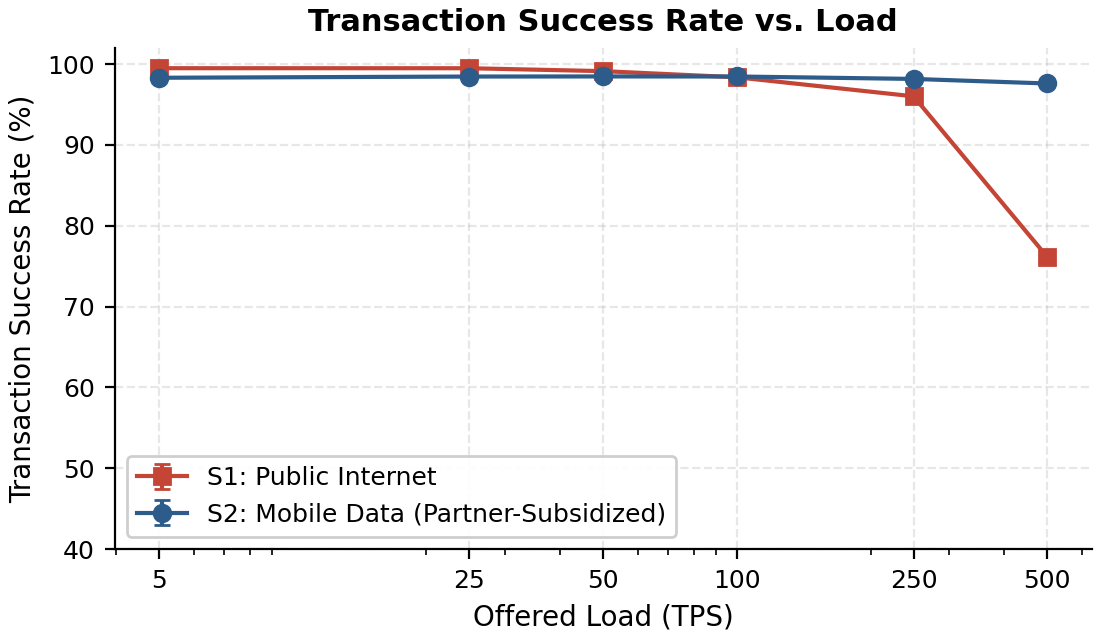
\includegraphics[width=0.85\textwidth]{fig6_success_rate.png}
\caption{نسبة نجاح المعاملة. يحافظ S2 على ~97.6\% عند 500 TPS، بينما ينهار S1 تحت الحمل.}
\label{fig:success}
\end{figure}

كما هو موضّح في الشكل~\ref{fig:latency}، يُظهر S2 زمن P95 مستقراً قرب 672 مللي ثانية عند 500 TPS. بينما يختبر S1 تدهوراً ملحوظاً، حيث يصل زمن P95 إلى ما يقارب 14.5 ثانية عند 500 TPS، مع تجاوز غالبية المعاملات الفاشلة لمهلة E2E البالغة 15 ثانية.

\begin{figure}[h]
\centering
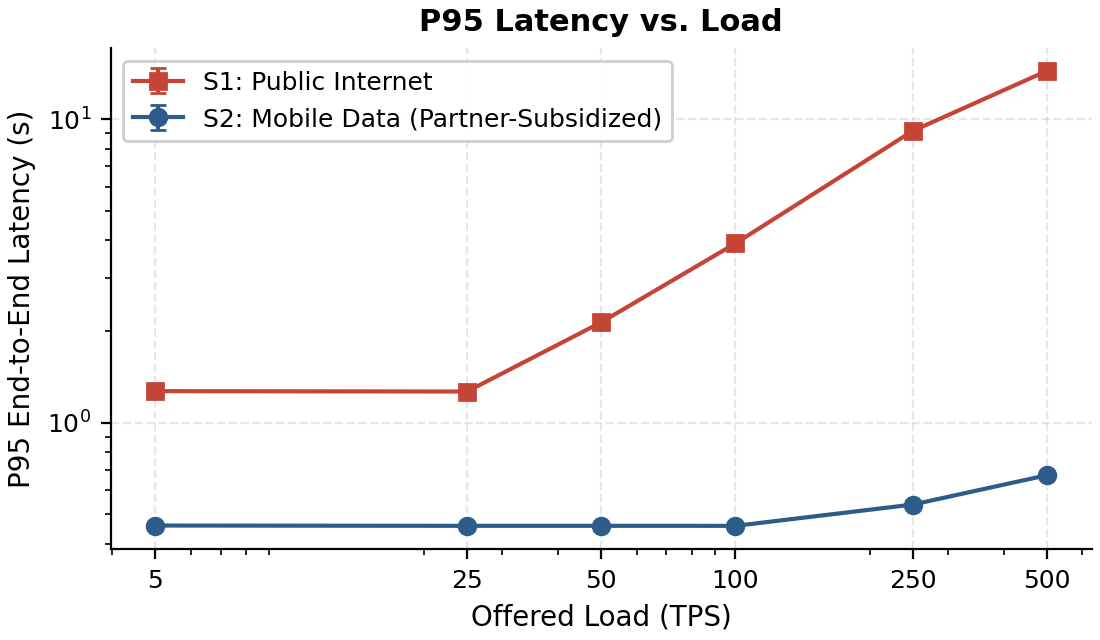
\includegraphics[width=0.85\textwidth]{fig7_p95_latency.png}
\caption{زمن استجابة P95. يبقى S2 مستقراً قرب 672 مللي ثانية عند 500 TPS؛ S1 يتضخّم تحت تدهور الحمل.}
\label{fig:latency}
\end{figure}

\begin{table}[h]
\centering
\caption{تفصيل الفشل عند 500 TPS ($N=10$، مجموع العدّات).}
\label{tab:failures}
\small
\begin{tabular}{@{}lcccc@{}}
\toprule
\textbf{السيناريو} & \textbf{نجاح} & \textbf{فقدان رفع} & \textbf{فقدان تنزيل} & \textbf{مهلة E2E} \\
\midrule
S1: الإنترنت العام & 76.15\% & 0 & 134{,}452 & 280{,}129 \\
S2: بيانات الهاتف & 97.61\% & 0 & 42{,}952 & 0 \\
\bottomrule
\end{tabular}
\end{table}

% ============================================================
\section{التحليل الاقتصادي ونموذج الاستدامة}
% ============================================================
الرؤية الاقتصادية الأساسية للمعمارية المُحدّثة هي أن حمولة مُحسّنة بدقة (180 بايت) تجعل توجيه بيانات الهاتف المحمول مستداماً اقتصادياً للمحفظة الشريكة. نُقسم هذا رسمياً عبر نموذج التكلفة التالي.

\subsection{نموذج التكلفة}
ليكن $N_{\mathrm{txn}}$ عدد المعاملات اليومية، $P_{\mathrm{size}} = 180$ بايت حجم الحمولة، $P_{\mathrm{data}}$ سعر البيانات لكل ميجابايت. التكلفة اليومية للبيانات:

\begin{equation}
C_{\mathrm{daily}} = \frac{N_{\mathrm{txn}} \cdot P_{\mathrm{size}}}{1{,}048{,}576} \cdot P_{\mathrm{data}}
\label{eq:cost}
\end{equation}

إيراد MDR اليومي (حيث $A_{\mathrm{avg}}$ متوسط المبلغ، $r_{\mathrm{MDR}}$ معدّل MDR):

\begin{equation}
R_{\mathrm{daily}} = N_{\mathrm{txn}} \cdot A_{\mathrm{avg}} \cdot r_{\mathrm{MDR}}
\label{eq:revenue}
\end{equation}

نسبة التكلفة من إيراد MDR:

\begin{equation}
\rho = \frac{C_{\mathrm{daily}}}{R_{\mathrm{daily}}} \times 100\%
\label{eq:ratio}
\end{equation}

\subsection{مثال عددي}
باستخدام مُعاملات واقعية للسوق اليمني:
\begin{itemize}
\item $N_{\mathrm{txn}} = 100{,}000$ معاملة يومية (محفظة شريكة وطنية)
\item $P_{\mathrm{size}} = 180$ بايت
\item $P_{\mathrm{data}} = \$1.00$ لكل MB (الحد الأعلى لـ Cable.co.uk لليمن)
\item $A_{\mathrm{avg}} = \$5$ (معاملة صغيرة)
\item $r_{\mathrm{MDR}} = 1\%$
\end{itemize}

\[
C_{\mathrm{daily}} = \frac{100{,}000 \times 180}{1{,}048{,}576} \cdot \$1.00 \approx \$17.17
\]

\[
R_{\mathrm{daily}} = 100{,}000 \cdot \$5 \cdot 0.01 = \$5{,}000
\]

\[
\rho = \frac{17.17}{5{,}000} \times 100\% \approx 0.34\%
\]

تستهلك تكلفة البيانات تقريباً 0.34\% من إيراد MDR، وهو أقل بكثير من عتبة 1\% التي تهدّد الاستدامة الاقتصادية. يُوضّح الشكل~\ref{fig:cost} حساسية هذه النسبة عبر أسعار بيانات وأحجام معاملات مختلفة.

\begin{figure}[h]
\centering
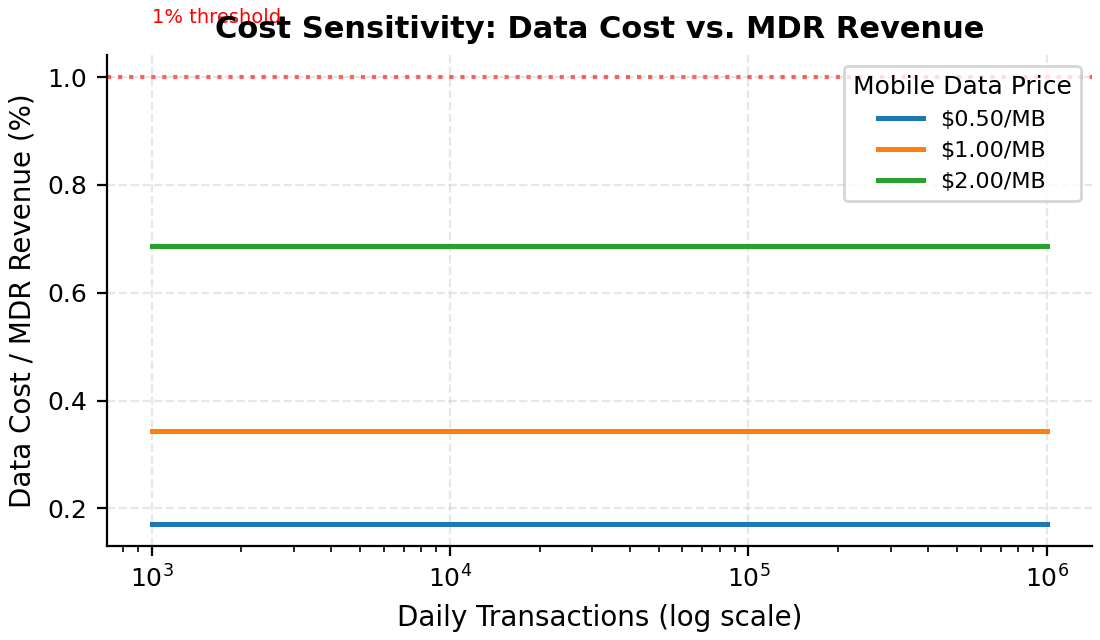
\includegraphics[width=0.85\textwidth]{fig8_cost_model.png}
\caption{حساسية التكلفة: تكلفة البيانات كنسبة من إيراد MDR، عبر أسعار بيانات الهاتف وأحمال المعاملات اليومية.}
\label{fig:cost}
\end{figure}

\subsection{مقارنة مع الأنظمة الموجودة}

\begin{table}[h]
\centering
\caption{مقارنة مع أنظمة الدفع الموجودة.}
\label{tab:comparison}
\small
\begin{tabular}{@{}p{2.7cm}p{2.3cm}p{2.3cm}p{2.7cm}p{2.3cm}@{}}
\toprule
\textbf{الميزة} & \textbf{أثير} & \textbf{M-Pesa} & \textbf{الكرمي} & \textbf{Kipaad} \\
\midrule
قابلية الأوفلاين & نعم (NFC) & جزئية (USSD) & جزئية (USSD) & نعم (NFC) \\
تكلفة الأجهزة & \$0 (SoftPOS) & \$0 & \$0 & POS مطلوب \\
النقل & بيانات الهاتف & USSD/SMS & USSD/SMS & NFC + SIM \\
متعدد المزوّدين & نعم & لا (Safaricom) & لا (بنك واحد) & لا \\
حجم الحمولة & 180 بايت & N/A & N/A & N/A \\
نموذج التكلفة & مدعوم من الشريك & يدفع المستخدم & يدفع المستخدم & يدفع المستخدم \\
\bottomrule
\end{tabular}
\end{table}

% ============================================================
\section{الخاتمة}
% ============================================================
فيما يتعلّق بأهداف التنمية الاقتصادية المستدامة، يُعدّ نظام أثير أحد حلول FinTech المبتكرة المُطوّرة خصيصاً للاقتصادات الهشّة وغير المطوّرة. لقد أظهرنا أن دمج NFC المبني على HCE مع توجيه بيانات الهاتف المحمول المُحسّن التكلفة يُنشئ أنظمة عملية وموثوقة، مُحقّقاً موثوقية 97.6\% عند 500 TPS في ظروف الإجهاد المُحاكاة. يتصدّى النظام لثلاث مجالات مهمة:

\begin{itemize}
\item \textbf{الموثوقية وقابلية التوسّع:} حيث أظهر مسار بيانات الهاتف المحمول نجاحاً 97.6\% عند 500 TPS، مُوفّراً بديلاً موثوقاً لأنظمة الإنترنت العام دون الحاجة إلى اتفاقيات APN خاصة مع المشغّلات.
\item \textbf{الحماية والسرّية:} حيث يُدمج النظام cryptogram بيومتري ونموذج Zero-Trust لضمان سلامة البيانات مع معالجة الانتحال والاحتيال.
\item \textbf{الأثر الاقتصادي والإدماج المالي:} من خلال ابتكار SoftPOS بدون تكلفة رأسمالية واتصال بيانات مدعوم من الشريك، يُقدّم النظام مزايا اقتصادية اجتماعية كبيرة.
\end{itemize}

% ============================================================
\section{العمل المستقبلي}
% ============================================================
تركّز أهدافنا قصيرة المدى على توسيع التعاون القطاعي لتطوير مشاريع تجريبية إضافية. نخطط لإجراء اختبارات ميدانية تتضمّن تعاونًا بين الجامعات والمحافظ الشريكة وشراكات قطاع عام-خاص. كما سنعمل على تأسيس شراكات مع مؤسسات مصرفية وهيئات تنظيمية لإنشاء مقترحات قابلة للتخصيص لتبنّي أطر التصريح الأوفلاين. أخيراً، ستخضع سمات الأمن المُؤسّسة في هذه الورقة لتحقق أمني رسمي باستخدام Tamarin Prover \cite{meier2013}، مما يُنتج إثباتات مُتحقَّق منها آلياً لمقاومة إعادة التشغيل وصحة المصادقة تحت نموذج تهديد Dolev-Yao، مما ينقل الادعاءات الأمنية من حجج قائمة على المعمارية إلى حجج قائمة على التحقق الرسمي.

% ============================================================
% References
% ============================================================
\begin{thebibliography}{99}

\bibitem{datareportal2024}
DataReportal, ``Digital 2024: Yemen,'' Kepios, 2024.

\bibitem{ookla2024}
Ookla, ``Speedtest Global Index: Yemen,'' 2024.

\bibitem{gsma2023}
GSMA, ``The State of Mobile Internet Connectivity Report 2023,'' London, U.K., 2023.

\bibitem{imf2022}
International Monetary Fund, ``Fintech in the Middle East and Central Asia,'' IMF Policy Paper No.~2022/004, 2022.

\bibitem{worldbank2023}
World Bank, ``Yemen Digital Economy Assessment,'' 2023.

\bibitem{brandpos2024}
BrandPOS, ``SoftPOS vs Traditional POS: A Complete Comparison,'' 2024.

\bibitem{oladapo2024}
O.~Oladapo \emph{et al.}, ``A review of tokenization and Host Card Emulation (HCE) in mobile payments,'' \emph{J. Cybersecurity Priv.}, vol.~4, no.~1, 2024.

\bibitem{hevner2004}
A.~R.~Hevner \emph{et al.}, ``Design science in information systems research,'' \emph{MIS Quart.}, vol.~28, no.~1, 2004.

\bibitem{peffers2007}
K.~Peffers \emph{et al.}, ``A design science research methodology for information systems research,'' \emph{JMIS}, vol.~24, no.~3, 2007.

\bibitem{mutawakel2024}
A.~Al-Mutawakel, ``Atheer Simulation Evaluation Artifact,'' GitHub Repository, 2024.

\bibitem{rfc8446}
E.~Rescorla, ``The Transport Layer Security (TLS) Protocol Version 1.3,'' RFC 8446, IETF, 2018.

\bibitem{meier2013}
S.~Meier \emph{et al.}, ``The TAMARIN prover for the symbolic analysis of security protocols,'' in \emph{Proc. CAV}, Springer, 2013.

\end{thebibliography}

\end{document}
